\usetikzlibrary{arrows.meta}
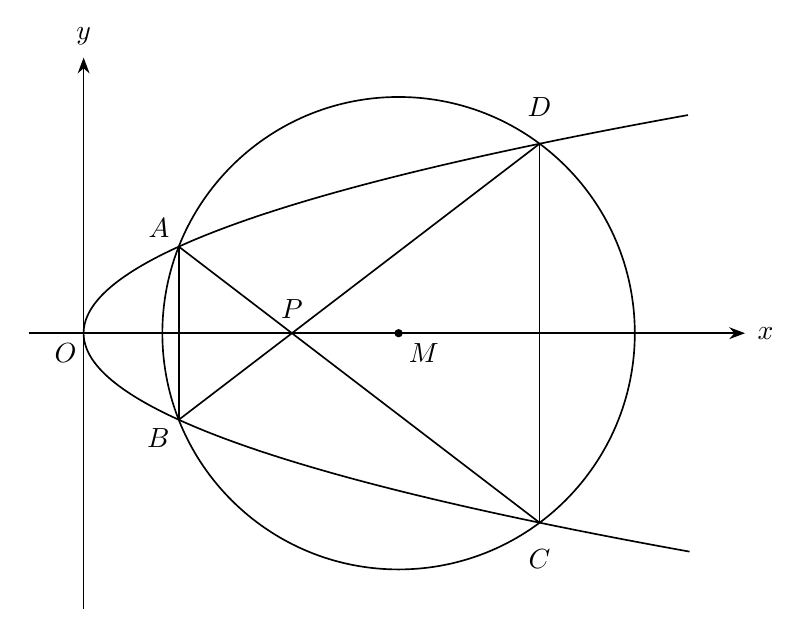
\begin{tikzpicture}[x=1cm,y=1cm,line width=.6pt,font=\normalsize,>=Stealth]
\coordinate (O) at (0,0);
\coordinate (M) at (4,0);
\coordinate (P) at (2.645751,0);
\coordinate (A) at (1.208712,1.099414);
\coordinate (B) at (1.208712,-1.099414);
\coordinate (C) at (5.791288,-2.406509);
\coordinate (D) at (5.791288,2.406509);
\draw[->] (-0.7,0)--(8.4,0);
\draw[->] (0,-3.5)--(0,3.5);
\draw[domain=-2.774:2.774,samples=241] plot ({\x*\x},{\x});
\draw (M) circle[radius=3];
\draw (A)--(B);
\draw (C)--(D);
\draw (A)--(C);
\draw (B)--(D);
\fill (M) circle[radius=1.5pt];
\node[anchor=north east,inner sep=0pt] at (-0.08,-0.12) {$O$};
\node[anchor=north west,inner sep=0pt] at (4.12,-0.12) {$M$};
\node[anchor=south,inner sep=0pt] at (2.645751,0.18) {$P$};
\node[anchor=south east,inner sep=0pt] at (1.1,1.2) {$A$};
\node[anchor=north east,inner sep=0pt] at (1.1,-1.2) {$B$};
\node[anchor=north,inner sep=0pt] at (5.79,-2.74) {$C$};
\node[anchor=south,inner sep=0pt] at (5.79,2.74) {$D$};
\node[anchor=west,inner sep=0pt] at (8.55,0) {$x$};
\node[anchor=south,inner sep=0pt] at (0,3.65) {$y$};
\end{tikzpicture}
